\documentclass[11pt]{article}
\usepackage[a4paper, margin=2.54cm]{geometry}
\usepackage[utf8]{inputenc}
\usepackage[spanish, mexico]{babel}
\usepackage[spanish]{layout}
\usepackage[article]{ragged2e}
\usepackage{textcomp}
\usepackage{amsmath}
\usepackage{amssymb}
\usepackage{amsfonts}
\usepackage{enumerate}
\usepackage{graphicx}

% ============================================================================
% ============================================================================
% ============================================================================

\title{
  Entrega N° 3 \\
  \large Modelos Físicos
}
\author{
  Farizano, Juan Ignacio \\
  \and
  Mellino, Natalia \\
  \and
  Prato, Valentina
}
\date{}

% ============================================================================
% ============================================================================
% ============================================================================

\begin{document}

\maketitle
\noindent\rule{\textwidth}{1pt}

\section*{Enunciado}
El péndulo simple de masa $m$ y longitud $l$ está suspendido de la masa $m_0$
que puede moverse libremente según la horizontal. El péndulo se suelta desde una
posición desplazada, y tiene lugar un movimiento acoplado de ambas masas.
Obtener las ecuaciones diferenciales del movimiento acoplado del sistema.
Determinar el período $\tau$ del péndulo para pequeñas oscilaciones, tómese
 $\sin \theta \approx 0$, $\cos \theta \approx 1$, y $\theta^2 \approx 0$.

 \begin{figure}[h!]
  \begin{center}
    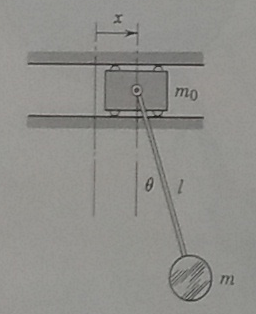
\includegraphics[width=0.20\linewidth]{pendulo.png}
  \end{center}
\end{figure}

\section*{Resolución}

Primero, fijamos nuestro sistema de referencia: el eje $x$ es positivo hacia
la derecha y el eje $y$ es positivo hacia abajo: el origen está situado a
la altura del centro de la masa $m_0$ y en en el lado izquierdo del gráfico,
donde la distancia $x$ que se ve en el gráfico es la distancia en el eje horizontal
desde el origen hacia el centro de la misma masa. \\

Ahora procedemos a plantear la ecuación de posición de la masa $m$, y a partir
de ella su vector velocidad:
\begin{align*}
  r &= (x + l \sin \theta; l \cos \theta) \\
  \dot{r} &= (\dot{x} + \dot{\theta} l \cos \theta; -l \dot{\theta} \sin \theta)
\end{align*}

Sabemos que la lagrangiana viene dada por:

\begin{equation*}
  L = T - V
\end{equation*}

Donde $T$ es la energía cinética y $V$ es la energía potencial.

\newpage

Calculamos $T$:
\begin{align*}
  T &= \frac{1}{2} m_0 \dot{x}^2 + \frac{1}{2} m \dot{r}^2 \\
\end{align*}

Donde: 
\begin{align*}
  \dot{r}^2 &= (\dot{x} + \dot{\theta} l \cos \theta)^2 + (-l \dot{\theta} \sin \theta)^2 \\
            &= \dot{x}^2 + 2 \dot{x}  \dot{\theta} l \cos \theta + \dot{\theta}^2 l^2 \cos^2 \theta
            + l^2 \dot{\theta}^2 \sin^2 \theta \\
            &= \dot{x}^2 + 2 \dot{x}  \dot{\theta} l \cos \theta + l^2 \dot{\theta}^2 (\cos^2 \theta + \sin^2 \theta) \\
            &= \dot{x}^2 + 2 \dot{x}  \dot{\theta} l \cos \theta + l^2 \dot{\theta}^2 \\
\end{align*}

Luego, calculamos $V$:

\begin{align*}
  V = m_0 g \underbrace{h_{x}}_{= 0} + m g h_{r} = m g (-l \cos \theta)
\end{align*}

Unimos todo

\begin{equation*}
  L = T - V = \frac{1}{2} m_0 \dot{x}^2 +
    \frac{1}{2} m (\dot{x}^2 + 2 \dot{x}  \dot{\theta} l \cos \theta + l^2 \dot{\theta}^2)
    + m g l \cos \theta \\
\end{equation*}

Como en este sistema la única fuerza que actúa es la de la gravedad que es
conservativa, podemos afirmar:

\begin{equation*}
  \frac{d}{dt} (\frac{\partial L}{\partial \dot{q}}) - \frac{\partial L}{\partial q} = 0
\end{equation*}

Calculamos para $\theta$:

\begin{align*}
  \frac{\partial L}{\partial \theta} &= -\frac{1}{2}m(2 \dot{x}  \dot{\theta} l \sin \theta)
    - m g l \sin \theta \\
    &= -ml\sin \theta (\dot{x} \dot{\theta} + g)
\end{align*}

\begin{align*}
  \frac{\partial L}{\partial \dot{\theta}} &= \frac{1}{2}m (2 \dot{x} l \cos \theta 
    + 2\dot{theta} l^2) \\
    &= ml(\dot{x} \cos \theta + \dot{\theta} l)
\end{align*}

\begin{align*}
  \frac{d}{dt} (\frac{\partial L}{\partial \dot{\theta}}) &= 
    ml(\ddot{x} \cos \theta - \dot{x} \dot{\theta} \sin \theta  + \ddot{\theta} l)
\end{align*}

\begin{align*}
  \frac{d}{dt} (\frac{\partial L}{\partial \dot{\theta}}) - \frac{\partial L}{\partial \theta} &=
  ml(\ddot{x} \cos \theta - \dot{x} \dot{\theta} \sin \theta  + \ddot{\theta} l)
  + ml( \dot{x} \dot{\theta} \sin \theta + g \sin \theta) \\
  &= ml (\ddot{x} \cos \theta - \dot{x} \dot{\theta} \sin \theta  + \ddot{\theta} l + \dot{x} \dot{\theta} \sin \theta + g \sin \theta) \\
  &= ml (\ddot{x} \cos \theta + \ddot{\theta} l + g \sin \theta) \\
  &= 0 \\
  &\underbrace{\iff}_{ml \neq 0} \\
  &\ddot{x} \cos \theta + \ddot{\theta} l + g \sin \theta = 0
\end{align*}

Cálculo auxiliar:
\begin{equation}
  \label{eq:aux}
  \ddot{x} \cos \theta + \ddot{\theta} l + g \sin \theta = 0
  \underbrace{\iff}_{\cos \theta \approx 1, \sin \theta \approx \theta}
  \ddot{x} + \ddot{\theta} l + g \theta = 0
  \iff \ddot{x} = - \ddot{\theta} l - g \theta
\end{equation}

Y calculamos para $x$:

\begin{equation*}
  \frac{\partial L}{\partial x} = 0
\end{equation*}

\begin{align*}
  \frac{\partial L}{\partial \dot{x}} &= 
    m_0 \dot{x} + \frac{1}{2}m(2\dot{x} + 2\dot{\theta} l \cos \theta) \\
    &= \dot{x} (m_0 + m) + ml\dot{\theta} \cos \theta  
\end{align*}

\begin{align*}
  \frac{d}{dt} (\frac{\partial L}{\partial \dot{x}}) - \frac{\partial L}{\partial x}
  =\frac{d}{dt} (\frac{\partial L}{\partial \dot{x}}) &= 
    \ddot{x}(m_0 + m) + ml\ddot{\theta} \cos \theta - ml \dot{\theta}^2 \sin \theta \\
    &= \ddot{x}(m_0 + m) + ml (\ddot{\theta} \cos \theta - \dot{\theta}^2 \sin \theta) = 0 \\
    &\underbrace{\Rightarrow}_{\cos \theta \approx 1, \theta^2 \approx 0} \\
    &\ddot{x}(m_0 + m) + ml\ddot{\theta} = 0  \\
    &\underbrace{\Rightarrow}_{\text{Ecuación (\ref{eq:aux})}} \\
    &(-l\ddot{\theta} - \theta g)(m_0 + m) +ml\ddot{\theta} = 0 \\
    &-l\ddot{\theta}m_0 - l\ddot{\theta}m - \theta g (m_0 + m) + ml\ddot{\theta} = 0 \\
    &l\ddot{\theta}m_0 + \theta g (m_0 + m) = 0 \\
    &l\ddot{\theta}m_0 = -\theta g (m_0 + m) \\
    &\ddot{\theta} = - \theta \frac{g}{l} \frac{m_0 + m}{m_0} \\
    &\ddot{\theta} + \theta \frac{g}{l} \frac{m_0 + m}{m_0} = 0
\end{align*}

A partir de reemplazar según los datos dados en el enunciado, obtenemos
una ecuación que se trata de la ecuación diferencial de un
Movimiento Armónico Simple de frecuencia angular.

\begin{equation*}
  \omega^2 = \frac{g}{l} \frac{m_0 + m}{m_0}
\end{equation*}

\begin{equation*}
  \tau = \frac{2\pi}{\omega} = 2\pi \sqrt{\frac{m_0}{m_0 + m} \frac{l}{g}}
\end{equation*}

\end{document}